% !TeX program = xelatex
% Extended abstract, Agent Evaluation Science symposium (2 pages excl. references).
% Build: cd paper/abstract && latexmk -xelatex main.tex
% Numbers come from ../../analysis/tables/numbers.tex (python -m src.report);
% never type a result into the prose. "% CHECK" marks sentences to re-read
% against the final numbers once all runs are scored.
\documentclass[11pt,a4paper]{article}
\usepackage{aes}
\usepackage{tabularx}
\usepackage{tikz}
\usetikzlibrary{arrows.meta,calc}

\graphicspath{{../../analysis/figures/}}
% Generated by src/report.py from analysis/results/. Do not edit by hand.
\newcommand{\nWorkshopsSmall}{30}
\newcommand{\nCallsSmall}{2,420}
\newcommand{\pctAnsweredSmall}{98.7\%}
\newcommand{\nCardsSmall}{360}
\newcommand{\blockCardsSmall}{2}
\newcommand{\nWorkshopsLarge}{120}
\newcommand{\nCallsLarge}{16,699}
\newcommand{\pctAnsweredLarge}{99.9\%}
\newcommand{\nCardsLarge}{1440}
\newcommand{\blockCardsLarge}{2}
\newcommand{\nWorkshopsFull}{60}
\newcommand{\nCallsFull}{13,353}
\newcommand{\pctAnsweredFull}{99.9\%}
\newcommand{\nCardsFull}{720}
\newcommand{\blockCardsFull}{2}
\newcommand{\nWorkshopsAll}{150}
\newcommand{\nCallsAll}{19,119}
\newcommand{\pctAnsweredAll}{99.7\%}
\newcommand{\nCardsAll}{1800}
\newcommand{\blockCardsAll}{4}
\newcommand{\nRuns}{10}
\newcommand{\chanceRules}{1.66}
\newcommand{\chanceSpec}{6.38}
\newcommand{\chanceDecision}{14\%}
\newcommand{\rulesQwenSmall}{3.5}
\newcommand{\rulesRangeQwenSmall}{2--4}
\newcommand{\specQwenSmall}{6.4}
\newcommand{\decisionQwenSmall}{4/10}
\newcommand{\modalQwenSmall}{6/10}
\newcommand{\recallGapQwenSmall}{-4.6}
\newcommand{\blockQwenSmall}{0/10}
\newcommand{\moreSupportiveQwenSmall}{47}
\newcommand{\moreCriticalQwenSmall}{43}
\newcommand{\rulesGemmaSmall}{2.8}
\newcommand{\rulesRangeGemmaSmall}{2--3}
\newcommand{\specGemmaSmall}{0.9}
\newcommand{\decisionGemmaSmall}{6/10}
\newcommand{\modalGemmaSmall}{6/10}
\newcommand{\recallGapGemmaSmall}{+1.1}
\newcommand{\blockGemmaSmall}{0/10}
\newcommand{\moreSupportiveGemmaSmall}{119}
\newcommand{\moreCriticalGemmaSmall}{0}
\newcommand{\rulesMistralSmall}{2.4}
\newcommand{\rulesRangeMistralSmall}{1--4}
\newcommand{\specMistralSmall}{5.4}
\newcommand{\decisionMistralSmall}{1/10}
\newcommand{\modalMistralSmall}{7/10}
\newcommand{\recallGapMistralSmall}{+6.5}
\newcommand{\blockMistralSmall}{2/10}
\newcommand{\moreSupportiveMistralSmall}{115}
\newcommand{\moreCriticalMistralSmall}{0}
\newcommand{\rulesQwenLargeLite}{1.45}
\newcommand{\rulesRangeQwenLargeLite}{1--3}
\newcommand{\specQwenLargeLite}{6.55}
\newcommand{\decisionQwenLargeLite}{0/20}
\newcommand{\modalQwenLargeLite}{20/20}
\newcommand{\recallGapQwenLargeLite}{+6.1}
\newcommand{\blockQwenLargeLite}{0/20}
\newcommand{\moreSupportiveQwenLargeLite}{108}
\newcommand{\moreCriticalQwenLargeLite}{85}
\newcommand{\rulesGemmaLargeLite}{1.0}
\newcommand{\rulesRangeGemmaLargeLite}{1--1}
\newcommand{\specGemmaLargeLite}{5.4}
\newcommand{\decisionGemmaLargeLite}{0/20}
\newcommand{\modalGemmaLargeLite}{20/20}
\newcommand{\recallGapGemmaLargeLite}{+6.1}
\newcommand{\blockGemmaLargeLite}{0/20}
\newcommand{\moreSupportiveGemmaLargeLite}{213}
\newcommand{\moreCriticalGemmaLargeLite}{27}
\newcommand{\rulesMistralLargeLite}{2.5}
\newcommand{\rulesRangeMistralLargeLite}{2--4}
\newcommand{\specMistralLargeLite}{5.9}
\newcommand{\decisionMistralLargeLite}{3/20}
\newcommand{\modalMistralLargeLite}{16/20}
\newcommand{\recallGapMistralLargeLite}{+4.5}
\newcommand{\blockMistralLargeLite}{0/20}
\newcommand{\moreSupportiveMistralLargeLite}{83}
\newcommand{\moreCriticalMistralLargeLite}{22}
\newcommand{\rulesQwenLargeFull}{1.9}
\newcommand{\rulesRangeQwenLargeFull}{1--3}
\newcommand{\specQwenLargeFull}{6.8}
\newcommand{\decisionQwenLargeFull}{0/20}
\newcommand{\modalQwenLargeFull}{20/20}
\newcommand{\recallGapQwenLargeFull}{+6.1}
\newcommand{\blockQwenLargeFull}{2/20}
\newcommand{\moreSupportiveQwenLargeFull}{11}
\newcommand{\moreCriticalQwenLargeFull}{215}
\newcommand{\rulesGemmaLargeFull}{1.35}
\newcommand{\rulesRangeGemmaLargeFull}{1--3}
\newcommand{\specGemmaLargeFull}{5.45}
\newcommand{\decisionGemmaLargeFull}{0/20}
\newcommand{\modalGemmaLargeFull}{20/20}
\newcommand{\recallGapGemmaLargeFull}{+6.1}
\newcommand{\blockGemmaLargeFull}{0/20}
\newcommand{\moreSupportiveGemmaLargeFull}{1}
\newcommand{\moreCriticalGemmaLargeFull}{239}
\newcommand{\rulesMistralLargeFull}{3.1}
\newcommand{\rulesRangeMistralLargeFull}{2--4}
\newcommand{\specMistralLargeFull}{5.5}
\newcommand{\decisionMistralLargeFull}{3/20}
\newcommand{\modalMistralLargeFull}{14/20}
\newcommand{\recallGapMistralLargeFull}{+3.1}
\newcommand{\blockMistralLargeFull}{0/20}
\newcommand{\moreSupportiveMistralLargeFull}{145}
\newcommand{\moreCriticalMistralLargeFull}{23}
\newcommand{\sizeDiffQwen}{-2.05}
\newcommand{\sizeCIQwen}{[-2.50, -1.55]}
\newcommand{\protocolDiffQwen}{+0.45}
\newcommand{\protocolCIQwen}{[+0.05, +0.80]}
\newcommand{\sizeDiffGemma}{-1.80}
\newcommand{\sizeCIGemma}{[-2.00, -1.50]}
\newcommand{\protocolDiffGemma}{+0.35}
\newcommand{\protocolCIGemma}{[+0.10, +0.65]}
\newcommand{\sizeDiffMistral}{+0.10}
\newcommand{\sizeCIMistral}{[-0.55, +0.75]}
\newcommand{\protocolDiffMistral}{+0.60}
\newcommand{\protocolCIMistral}{[+0.20, +0.95]}
\newcommand{\nRunsLarge}{120}
\newcommand{\lrcLarge}{110}
\newcommand{\enrolLowLarge}{110}
\newcommand{\humanSelfRules}{3}
\newcommand{\humanSelfSpec}{10}
\newcommand{\humanChangedRules}{4}
\newcommand{\shiftItemsQwenSmall}{5.5}
\newcommand{\shiftStricterQwenSmall}{2.0}
\newcommand{\shiftPermissiveQwenSmall}{3.5}
\newcommand{\rulesShiftedQwenSmall}{1.8}
\newcommand{\shiftSameQwenSmall}{10\%}
\newcommand{\shiftItemsGemmaSmall}{5.3}
\newcommand{\shiftStricterGemmaSmall}{1.6}
\newcommand{\shiftPermissiveGemmaSmall}{3.7}
\newcommand{\rulesShiftedGemmaSmall}{1.6}
\newcommand{\shiftSameGemmaSmall}{7\%}
\newcommand{\shiftItemsMistralSmall}{5.7}
\newcommand{\shiftStricterMistralSmall}{2.0}
\newcommand{\shiftPermissiveMistralSmall}{3.7}
\newcommand{\rulesShiftedMistralSmall}{2.3}
\newcommand{\shiftSameMistralSmall}{11\%}
\newcommand{\shiftItemsQwenLargeLite}{2.5}
\newcommand{\shiftStricterQwenLargeLite}{1.4}
\newcommand{\shiftPermissiveQwenLargeLite}{1.1}
\newcommand{\rulesShiftedQwenLargeLite}{1.0}
\newcommand{\shiftSameQwenLargeLite}{3\%}
\newcommand{\shiftItemsGemmaLargeLite}{0.9}
\newcommand{\shiftStricterGemmaLargeLite}{0.0}
\newcommand{\shiftPermissiveGemmaLargeLite}{0.9}
\newcommand{\rulesShiftedGemmaLargeLite}{0.0}
\newcommand{\shiftSameGemmaLargeLite}{0\%}
\newcommand{\shiftItemsMistralLargeLite}{3.0}
\newcommand{\shiftStricterMistralLargeLite}{1.4}
\newcommand{\shiftPermissiveMistralLargeLite}{1.6}
\newcommand{\rulesShiftedMistralLargeLite}{1.3}
\newcommand{\shiftSameMistralLargeLite}{5\%}
\newcommand{\shiftItemsQwenLargeFull}{4.2}
\newcommand{\shiftStricterQwenLargeFull}{3.7}
\newcommand{\shiftPermissiveQwenLargeFull}{0.5}
\newcommand{\rulesShiftedQwenLargeFull}{2.8}
\newcommand{\shiftSameQwenLargeFull}{15\%}
\newcommand{\shiftItemsGemmaLargeFull}{1.8}
\newcommand{\shiftStricterGemmaLargeFull}{0.7}
\newcommand{\shiftPermissiveGemmaLargeFull}{1.1}
\newcommand{\rulesShiftedGemmaLargeFull}{0.1}
\newcommand{\shiftSameGemmaLargeFull}{0\%}
\newcommand{\shiftItemsMistralLargeFull}{2.2}
\newcommand{\shiftStricterMistralLargeFull}{1.4}
\newcommand{\shiftPermissiveMistralLargeFull}{0.8}
\newcommand{\rulesShiftedMistralLargeFull}{1.0}
\newcommand{\shiftSameMistralLargeFull}{4\%}
\newcommand{\humanShiftItems}{10}
\newcommand{\humanShiftStricter}{7}
\newcommand{\humanShiftPermissive}{3}
\newcommand{\humanSensitiveStricter}{5}
\newcommand{\nSensitive}{7}
\newcommand{\nRunsFullAll}{60}
\newcommand{\lrcFull}{54}
\newcommand{\enrolLowFull}{54}
\newcommand{\baseLrcFull}{58}
\newcommand{\supportCardsFull}{0}
\newcommand{\humanSupportCards}{4}
\newcommand{\humanSupportWithReservationsCards}{2}
\newcommand{\humanObjectNoBlockCards}{2}
\newcommand{\humanBlockCards}{2}
\newcommand{\reservationsFull}{97\%}
\newcommand{\changedQwenSmall}{23\%}
\newcommand{\changedGemmaSmall}{20\%}
\newcommand{\changedMistralSmall}{29\%}
\newcommand{\changedQwenLargeLite}{10\%}
\newcommand{\changedGemmaLargeLite}{3\%}
\newcommand{\changedMistralLargeLite}{13\%}
\newcommand{\changedQwenLargeFull}{13\%}
\newcommand{\changedGemmaLargeFull}{3\%}
\newcommand{\changedMistralLargeFull}{7\%}
% aliases: small tier
\newcommand{\rulesQwen}{\rulesQwenSmall}
\newcommand{\rulesRangeQwen}{\rulesRangeQwenSmall}
\newcommand{\specQwen}{\specQwenSmall}
\newcommand{\decisionQwen}{\decisionQwenSmall}
\newcommand{\modalQwen}{\modalQwenSmall}
\newcommand{\recallGapQwen}{\recallGapQwenSmall}
\newcommand{\blockQwen}{\blockQwenSmall}
\newcommand{\moreSupportiveQwen}{\moreSupportiveQwenSmall}
\newcommand{\moreCriticalQwen}{\moreCriticalQwenSmall}
\newcommand{\rulesGemma}{\rulesGemmaSmall}
\newcommand{\rulesRangeGemma}{\rulesRangeGemmaSmall}
\newcommand{\specGemma}{\specGemmaSmall}
\newcommand{\decisionGemma}{\decisionGemmaSmall}
\newcommand{\modalGemma}{\modalGemmaSmall}
\newcommand{\recallGapGemma}{\recallGapGemmaSmall}
\newcommand{\blockGemma}{\blockGemmaSmall}
\newcommand{\moreSupportiveGemma}{\moreSupportiveGemmaSmall}
\newcommand{\moreCriticalGemma}{\moreCriticalGemmaSmall}
\newcommand{\rulesMinistral}{\rulesMistralSmall}
\newcommand{\rulesRangeMinistral}{\rulesRangeMistralSmall}
\newcommand{\specMinistral}{\specMistralSmall}
\newcommand{\decisionMinistral}{\decisionMistralSmall}
\newcommand{\modalMinistral}{\modalMistralSmall}
\newcommand{\recallGapMinistral}{\recallGapMistralSmall}
\newcommand{\blockMinistral}{\blockMistralSmall}
\newcommand{\moreSupportiveMinistral}{\moreSupportiveMistralSmall}
\newcommand{\moreCriticalMinistral}{\moreCriticalMistralSmall}
\newcommand{\nWorkshops}{\nWorkshopsSmall}
\newcommand{\nCalls}{\nCallsSmall}
\newcommand{\pctAnswered}{\pctAnsweredSmall}
\newcommand{\nCards}{\nCardsSmall}
\newcommand{\blockCards}{\blockCardsSmall}


\title[Synthetic Stakeholders?]{Synthetic Stakeholders? Agreement and Stability of Open-Weight LLM Agent Panels in Participatory Model Selection}

\aesauthor[affil={1},corresponding]{Tereza Bla\v{z}kov\'a}
\aesaffiliation{1}{Center for Social Data Science, University of Copenhagen}
\aesemails{\aesemail{tereza.blazkova@sodas.ku.dk}}

\begin{document}
\maketitle

\begin{abstract}
LLM agents are proposed as synthetic participants, but rarely tested against a real deliberation.
We replay a workshop in which 12 students and advisors set the rules for selecting a university dropout early-warning model with 12-agent panels from three open-weight model families, at two sizes and under an abridged or the full workshop protocol (\nWorkshopsAll{} workshops).
Small models matched \rulesMistralSmall--\rulesQwenSmall{} of the 7 rules the humans set (random panels: \chanceRules{}; the same humans before deliberation: \humanSelfRules{}); at 24--27B, two of three families chose the same configuration in every run while matching about as many rules as random panels, the full protocol helped only slightly, and panels almost never objected (\blockCardsAll{} blocking votes in \nCardsAll{}): synthetic panels are more uniform and agreeable than the one human panel we can compare them with.
\end{abstract}

\section{Motivation}
Participatory AI asks affected people to shape algorithmic systems \citep{birhanePowerPeopleOpportunities2022,delgadoParticipatoryTurnAI2023}; because this is slow and costly, LLM-simulated participants are proposed as substitutes \citep{argyle2023outofone,aher2023using}, although they misrepresent and flatten the groups they stand in for \citep{santurkar2023whose,wang2025misportray} and, as simulated users, are ``excessively cooperative'' and ``stylistically uniform'' \citep{zhou2026sim2real}.
Whether they are valid proxies is an open question for agent evaluation \citep{chen2026trends}; we compare synthetic stakeholder panels with what one real participatory process \emph{produced}: binding selection rules and the model they select.

\begin{figure}[b]
  \centering
  % Design diagram: the human workshop (top lane) and a synthetic panel (bottom
% lane) pass through the same stages. The two are compared at the baseline and
% at the endline survey (and on the change between them). The grey stages are
% not part of the simulated workshop: the endline medians are turned into rules
% and a model programmatically, identically in both lanes.
% Edit labels freely; layout is a 6-column grid.
\begin{tikzpicture}[
    font=\scriptsize,
    stage/.style={rectangle, rounded corners=2pt, align=center, minimum height=9mm,
                  text width=20mm, inner sep=1.5pt, draw=#1!75!black, fill=#1!10, line width=0.5pt,
                  execute at begin node={\hyphenpenalty=10000\relax}},
    derived/.style={rectangle, rounded corners=2pt, align=center, minimum height=9mm,
                  text width=20mm, inner sep=1.5pt, draw=black!30, fill=black!4, text=black!55,
                  line width=0.5pt, dashed, execute at begin node={\hyphenpenalty=10000\relax}},
    flow/.style={-{Stealth[length=1.5mm]}, line width=0.5pt, draw=black!50},
    gflow/.style={-{Stealth[length=1.5mm]}, line width=0.5pt, draw=black!25},
    cmp/.style={{Stealth[length=1.6mm]}-{Stealth[length=1.6mm]}, line width=0.9pt, draw=black},
    cmplabel/.style={font=\tiny\bfseries, fill=white, inner sep=1pt, align=center},
    lane/.style={font=\scriptsize\bfseries, anchor=east, align=right},
    note/.style={font=\tiny, text=black!60, fill=white, inner sep=1pt, align=center},
  ]
  \def\dx{22.5mm}
  \def\dy{15mm}
  \colorlet{hum}{black!45}
  \colorlet{syn}{aespurple}

  % ---- human lane ----
  \node[stage=hum] (h1) at (0,0)      {9 students\\+ 3 advisors};
  \node[stage=hum] (h2) at (\dx,0)    {Baseline survey};
  \node[stage=hum] (h3) at (2*\dx,0)  {3\,h deliberation};
  \node[stage=hum] (h4) at (3*\dx,0)  {Endline survey};
  \node[derived] (h5) at (4*\dx,0)    {Median rules};
  \node[derived] (h6) at (5*\dx,0)    {Logistic regression\\+ performance};

  % ---- synthetic lane ----
  \node[stage=syn] (s1) at (0,-\dy)     {12 LLM agents\\(fictional personas)};
  \node[stage=syn] (s2) at (\dx,-\dy)   {Baseline survey};
  \node[stage=syn] (s3) at (2*\dx,-\dy) {same protocol\\(scripted)};
  \node[stage=syn] (s4) at (3*\dx,-\dy) {Endline survey};
  \node[derived] (s5) at (4*\dx,-\dy)   {Median rules};
  \node[derived] (s6) at (5*\dx,-\dy)   {Selected model};

  \foreach \i/\j in {1/2,2/3,3/4} {
    \draw[flow] (h\i) -- (h\j);
    \draw[flow] (s\i) -- (s\j);
  }
  \foreach \i/\j in {4/5,5/6} {
    \draw[gflow] (h\i) -- (h\j);
    \draw[gflow] (s\i) -- (s\j);
  }

  % the comparisons: the same survey, before and after deliberation
  \draw[cmp] (h2.south) -- node[cmplabel] {compare\\baseline} (s2.north);
  \draw[cmp] (h4.south) -- node[cmplabel] {compare\\endline} (s4.north);

  % lane labels, the manipulated factor, the programmatic (not simulated) steps
  \node[lane, text=black!70] at ($(h1.west)+(-1.5mm,0)$) {Human\\workshop};
  \node[lane, text=aespurple!80!black] at ($(s1.west)+(-1.5mm,0)$) {Synthetic\\panel};
  \node[note, text=aespurple!80!black, anchor=north] at ($(s2.south)!0.5!(s4.south)+(0,-0.8mm)$)
       {3 open-weight families (Qwen 3.5 27B, Gemma 3 27B, Mistral Small 3.2 24B) $\times$ 20 seeded runs};
  \node[note, text=black!50, anchor=south] at ($(h5.north)!0.5!(h6.north)+(0,0.8mm)$)
       {not simulated: same median rule and selection algorithm in both lanes};
\end{tikzpicture}

  \caption{Design. Both lanes share the survey, aggregation and selection algorithm; within each setting, only the model family varies.}
  \label{fig:design}
\end{figure}

\section{Human reference and design}
In a three-hour deliberative workshop at a Danish university \citep{blazkova2026participatory}, 9 students and 3 student advisors answered a survey before and after deliberation \citep{fishkin2009people}, pricing each step on two ladders in students identified per 100: adding data (course performance, enrolment, LMS activity, sensitive attributes) and lowering explainability (from a credit rule to a neural network).
Their endline medians, applied to all candidate models on the 2021 cohort, selected logistic regression on credits and performance (recall 62.3\% vs.\ 23.5\% for the current credit rule).
This workshop is one draw, not a ground truth: how much workshops with similar or the same people would differ is unknown, and its own participants' pre-deliberation rules match their final ones on only \humanSelfRules{} of 7. We therefore report agreement with this reference next to random panels and the same humans before deliberation.
Synthetic panels replay this process (Figure~\ref{fig:design}) with 12 fictional personas matching the published role and demographic mix, the verbatim survey and a scripted facilitator, in a \emph{lite} protocol (one plenary round) and the \emph{full} human protocol (tables, plenary, 1-2-4-All).
Families are Qwen 3.5, Gemma 3 and Mistral (Ministral 3, Mistral Small 3.2; 4-bit, temperature~1), small (3--4B, lite, 10 runs) and large (24--27B, lite and full, 20 runs), with seeded speaking orders matched across families.
The scoring checklist and a random-panel reference were fixed before any model output; no personal data or transcripts were used, and \pctAnsweredAll{} of choice items were answered.

\section{Results}
\begin{figure}[t]
  \centering
  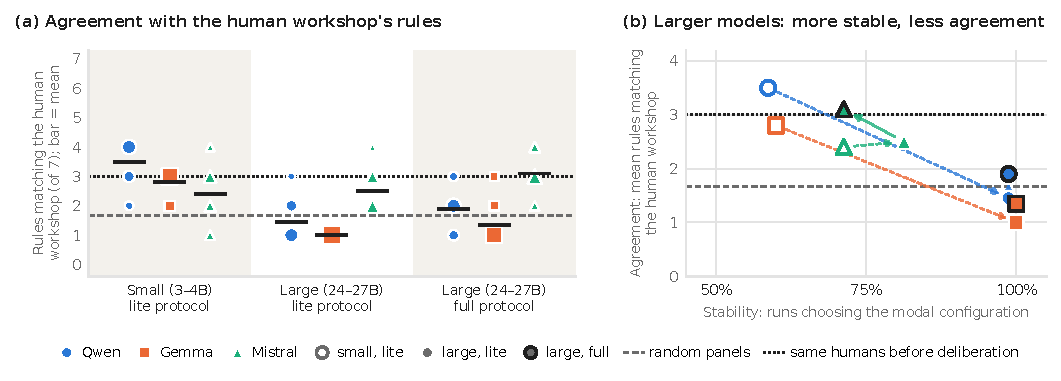
\includegraphics[width=\linewidth]{fig_settings.pdf}
  \caption{(a)~Selection rules matching the human workshop per run (marker area = runs; bar = mean). (b)~Agreement against stability (share of runs choosing the family's modal configuration); arrows go from small to large models and from lite to full. Dashed: random panels; dotted: the same humans before deliberation.}
  \label{fig:settings}
\end{figure}

% Table 1 (all nine settings) moved out for the 2-page version: ../../analysis/tables/table_main.tex

Small panels recover more selection rules than random panels, but at most half, and the families err in different directions; they select the human model in \decisionQwenSmall{}, \decisionGemmaSmall{} and \decisionMistralSmall{} runs (Qwen, Gemma, Mistral; random panels \chanceDecision{}), large panels in \decisionQwenLargeLite{} to \decisionMistralLargeLite{} in either protocol.
Scaling up makes panels more stable but further from the human rules (Figure~\ref{fig:settings}): Qwen and Gemma panels choose the same configuration in every run while their rule agreement falls to or below random-panel level (size effect $\sizeDiffQwen$ $\sizeCIQwen$ and $\sizeDiffGemma$ $\sizeCIGemma$ rules; Mistral $\sizeDiffMistral$ $\sizeCIMistral$).
Large panels price admissions and enrolment data at a small or moderate gain in \enrolLowLarge{} of \nRunsLarge{} runs (humans: large), the threshold that flips the selection in the human study's robustness analysis; \lrcLarge{} of \nRunsLarge{} large panels thus select logistic regression with enrolment data ($+6.1$~pp recall) instead of the human model.
The full protocol raises agreement slightly but reliably (Qwen $\protocolDiffQwen$ $\protocolCIQwen$, Gemma $\protocolDiffGemma$ $\protocolCIGemma$, Mistral $\protocolDiffMistral$ $\protocolCIMistral$) and never restores the human decision for Qwen or Gemma.

\paragraph{Limitations and implications.}
With one human workshop, agreement is distance to one reference, not validity; two descriptive findings do not depend on it: large Qwen and Gemma panels repeat one choice in every run while one human group revised \humanChangedRules{} of 7 rules in an afternoon, and panels almost never dissent (\blockCardsAll{} blocking votes in \nCardsAll{}; humans: a blocking minority), the cooperative-AI risk of manufactured consensus \citep{dafoe2020open,tessler2024habermas}.

\bibliography{references}

\end{document}
